%%
%% Author: thompson
%% 25.11.17
%%

% Preamble
\documentclass[11pt]{article}

% Packages
\usepackage{a4wide}
\usepackage[ngerman]{babel}
\usepackage[utf8]{inputenc}

\usepackage{scrextend}
\usepackage{enumerate}
\usepackage{graphicx}


% Document
\begin{document}

    \graphicspath{{PictureDoc/}}


    \section{OMNeT++}
    \subsection{Q\&A}

    \begin{enumerate}[\thesubsection .1]
        \item Wie wird eine Topologie erstellt und dessen Funktionalität realisiert?\\
        Eine Topologie, sprich eine Simulation wird in OMNeT++ mithilfe mehrerer Datentypen definiert. Es gibt:
        \begin{enumerate}[$\circ$]
            \item .NED - \textbf{NE}twork \textbf{D}escription File
            In diesen beschreibt man, wie der Name bereits verät, das Netzwerk mit all dessen Knoten, Empfängern wie Sendern.
            Neben den DataNodes beschreibt man auch den groben Funktionsumfang, etwa wann Daten gesendet werden sowie Delay.
            Mithilfe 2er Modi: Source und Design lässt sich das Netzwerk graphisch als auch programmiertechnisch beliebig anpassen
            \item .CC - C++ Datensätze
            In diesen beschreibt man die Subfunktionen e.g. das Verhalten aller Instanzen innerhalb des Netzwerkes.
            Für gewöhnlich bedient man sich vordefinierten Spezifikationen wie cMessage oder cSimpleModule, von welchen
            die eigenen Klassen erben.
            \item .INI - Initialisierungsdatei
            Diese beschreibt das zu simulierende Netzwerk, definiert im .NED-File.
            \emph{Es gilt die Klasse anzugeben, nicht den Dateinamen.}
        \end{enumerate}

        \item Wie kompiliert und startet eine Simulation?\\
        Prinzipiell mithilfe des RUN-Buttons der IDE.

        Für gewöhnlich gilt es mithilfe von cpp-makemake ein File zu erstellen, welches dann ausgeführt wird.
        Dieses orientiert sich an der jeweiligen omnetpp.ini-Datei, worin die auszuführenden Daten spezifiziert sind.
        Ähnlich einer Kettenreaktion wird dann der Rest ausgelesen, kompiliert und ausgeführt.

        \item Wie fügt man folgende hinzu:
        \begin{addmargin}[1em]{1em}
            - Graphische Elemente: \\
            - Ausgaben zur Fehlersuche: \\
            - Zustandsvariablen: \\
            - (Zufällige) Parameter:
        \end{addmargin}


        \item Wie setzt man Vererbung, Verzögerung, Zeitüberschreitung um oder hebt diese auf?\\


        \item Wie funktionieren Netzwerktopologien mit mehr als 2 Knoten?\\


        \item Wie wird ein eigenes Nachrichtenformat definiert und wie werden sie verwendet?\\


        \item Statistiken, Auswertung und Visualisierung - Wie setzt man sie um?\\

        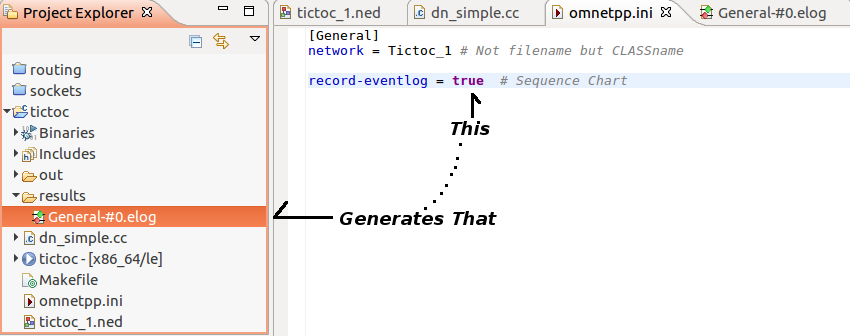
\includegraphics[width=\textwidth]{charting1.png}

        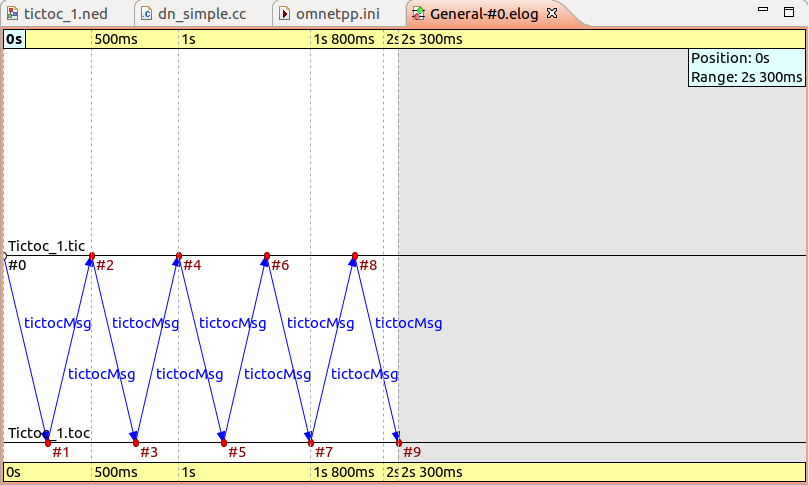
\includegraphics[width=\textwidth]{charting2.png}


    \end{enumerate}
\end{document}